\documentclass[12pt,ngerman]{scrartcl}

\usepackage[left=5mm,right=5mm,top=5mm,bottom=5mm]{geometry}

\pagestyle{empty}
\usepackage{tikz}

\usetikzlibrary{decorations.pathmorphing}
\tikzset{snake it/.style={decorate, decoration=snake}}

\begin{document}

\begin{tikzpicture}

\node[anchor=north west,inner sep=0](frame1) at (0,23){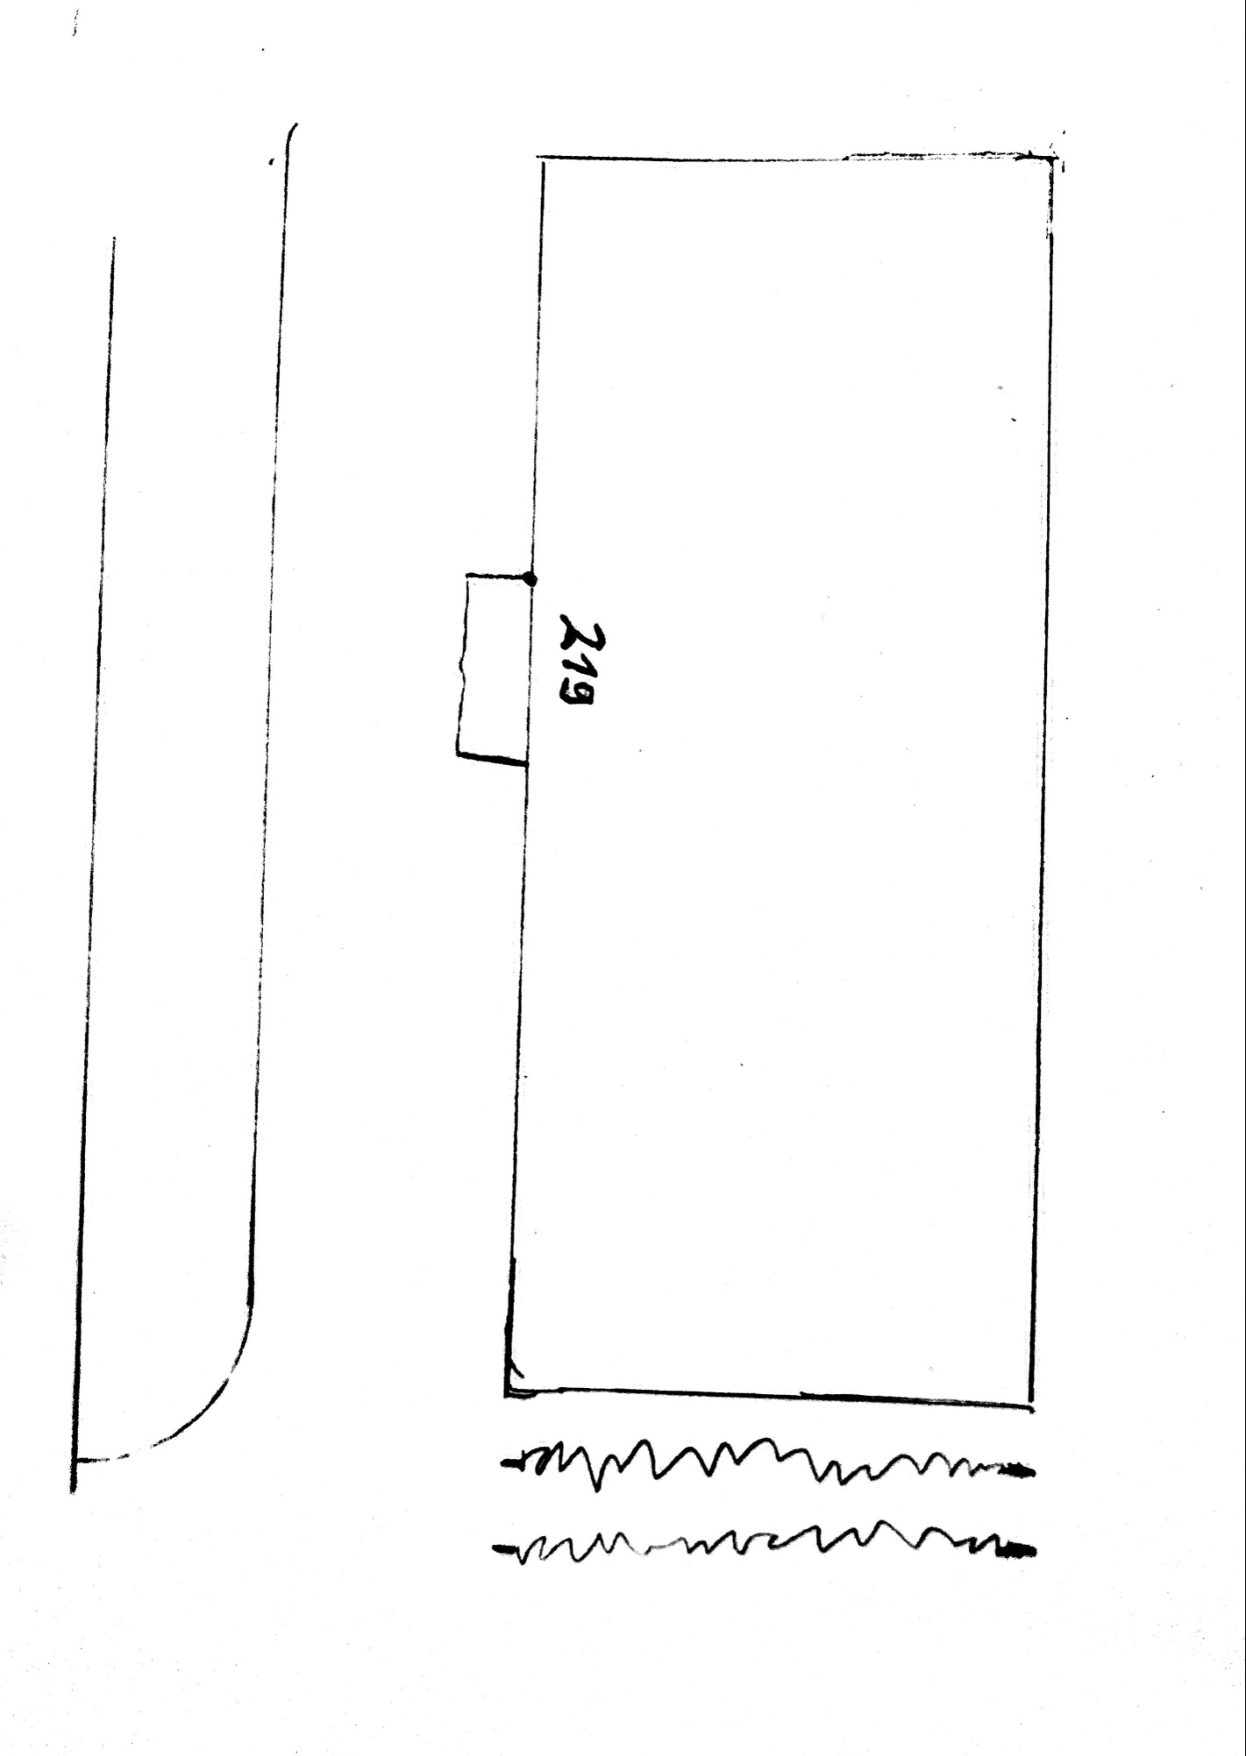
\includegraphics[width=15cm,angle=180]{Scan.pdf}};

\draw[help lines,blue] (0,0) grid (18,24);
\foreach \xtick in {1,...,18} {\pgfmathsetmacro\result{\xtick} \node at (\xtick,-0.5) {\pgfmathprintnumber{\result}}; }
\foreach \ytick in {0,...,23} {\pgfmathsetmacro\result{\ytick} \node at (0.25,\ytick) {\pgfmathprintnumber{\result}}; }

\draw[very thick,red] (2.35,3.8) -- (2.55,18.85) -- (8.9,18.7) -- (8.5,3.7) -- cycle;

\draw[very thick,red] (11.5,3.3) -- (12,17.5) arc (180:88:2) -- (13.6,4.8);

\node[rotate=90,red] at (7,10) {\LARGE\bfseries 219};

\draw[red,very thick,snake it] (2.5,19.5) -- (9,19.5);

\draw[red,very thick,snake it] (2.5,20.5) -- (9,20.5);

\end{tikzpicture}


\end{document}